\documentclass[pdf]{beamer}
\mode<all>{\usetheme{Warsaw} \useoutertheme{default}}
\mode<handout>{\usecolortheme{seagull}}
\usenavigationsymbolstemplate{}

\title{Introduction to Commutative Algebra}
\subtitle{and affine algebraic varieties}
\author{Amal M}
\date{\today}

\begin{document}

\AtBeginSection[]{
\begin{frame}{Table of Contents}
	\tableofcontents[currentsection]
\end{frame}
}

\begin{frame}
    \thispagestyle{empty}
    \titlepage
\end{frame}
\addtocounter{framenumber}{-1}

\begin{frame}{Table of Contents}
    \tableofcontents
\end{frame}

%%%%%%%%%%%%%%%%%%%%%%%%%%%%%%%%%%%%%%%%%%%%%%%%%%

\section{Introduction}
\subsection{2 min}


\begin{frame}
    \frametitle{Introduction}
    The Plan
    \begin{itemize}
        \item Study undergraduate algebraic geometry 
        \item Read and do the exercies from Atiyah-Macdonald, Introduction to Commutative Algebra
        \item Read first chapter of Hartshorne's Algebraic Geometry
    \end{itemize}
\end{frame}


\section{Algebraic Varieties}
\subsection{3 min}

\begin{frame}
    \frametitle{Curves}
    $y^2 = x^3 − 3x + 5$ is a polynomial in $\mathbb{R}[x,y]$. The set of zeros of this polynomial looks like this
    \begin{center}
        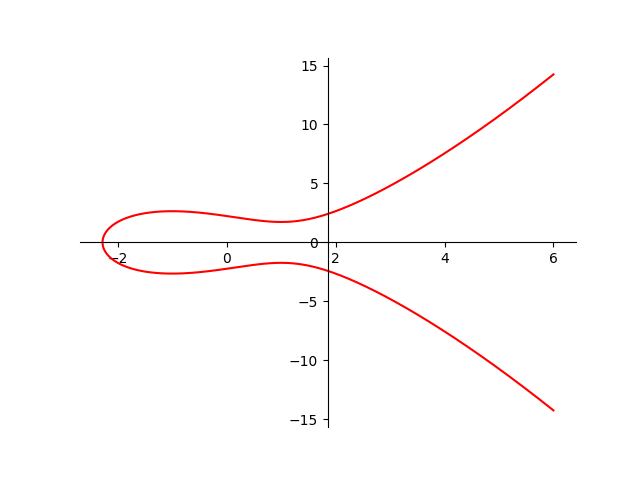
\includegraphics[height=2in]{ell_curv1.png}
    \end{center}
\end{frame}

\begin{frame}
    \frametitle{Polynomial Ring}
    Given a algebraicaly closed field $k$ we can form the polynomial ring in $n$ indeterminants
    $$k[x_1, \cdots, x_n]$$
    Every polynomial $p(x_1, \cdots, x_n) \in k[x_1, \cdots, x_n]$ can be thought of as a mapping from $k^n \rightarrow k$.
    We call $k^n$ the \textit{affine $n$-space} and denote it by $\mathbb{A}^n_k$.
\end{frame}

\begin{frame}
    \frametitle{Affine Algebraic Varieties}
    $S$ is a set of polynomial in $k[x_1, \cdots, x_n]$. $V(S)$ is points in $\mathbb{A}^n_k$ at which every polynomial in $S$ \textit{vanishes}. $V(S)$ is called the \textit{affine algebraic variety}.
\end{frame}    

\section{Nullstellensatz}
\subsection{5 min}

\begin{frame}
    \frametitle{The Coordinate Ring}
    Given a variety $V$ in $\mathbb{A}^n_k$ the \textit{ideal of a variety} is the ideal $I(V)$ which consists of all polynomials in $k[x_1, \cdots, x_n]$ that vanish on $V$. The Coordinate ring of a variety is the ring
    $$P(X) = k[x_1, \cdots, x_n]/I(X)$$
\end{frame}

\begin{frame}
    \frametitle{Hilbert's Nullstellensatz}
    \center Nullstellensatz means the theorem of zeros.
    \begin{center}
    \begin{tabular}{c | c}
        \large{\textbf{Algebra}} & \large{\textbf{Geometry}} \\
        $k[x_1, \cdots, x_n]$ & $\mathbb{A}^n_k \cong k^n$ \\
        $I(V)$ & $V(I)$ \\
        $(x - a_1, \cdots, x - a_n)$ & the point $(a_1, \cdots, a_n)$
    \end{tabular}
\end{center}
\end{frame}

\begin{frame}
    \frametitle{Algebraic - Geometry}
    There is a connection between geometric objects such as curves and the algebraical objects like a ring. 
\end{frame}

\begin{frame}
    \frametitle{Regular mappings}
    Explain polynomial mapping/regular mapping between varieties
\end{frame}

\section{Commutative Algebra}
\subsection{2 min}

\begin{frame}
    \frametitle{What sort of Commutative Algebra do we use?}
    What sort of commutative algebra machinery do we use: (Do not explain any of these. Point out where you use them instead)
    \begin{enumerate}
        \item Modules
        \item Tensor products
        \item Exact sequnces
        \item Direct Limits
    \end{enumerate}
\end{frame}

\section{Zariski Topology}
\subsection{3 min}

\begin{frame}
    \frametitle{Zariski}
    Talk about the prime spectrum and the Zariski Topology what sort of machinery would that use? 
\end{frame}

\begin{frame}
    \frametitle{Constructible Topology}
    You can have another topology called the Constructible Topology
\end{frame}

\section{Presheaf and Sheaf}
\subsection{4 min}

\begin{frame}
    \frametitle{Presheaf and Sheaf}
     Definiton of a Presheaf and Sheaf 
 \end{frame}

 \section{Applications}
 \subsection{1 min}

 \begin{frame}
     \frametitle{Applications of Algebraic Geometry}
    Do you really want applications? You could mention in passing string theory, arithmetic geometry, proof of the Fermat’s last theorem etc… 
\end{frame}

\section{Conclusion}

\begin{frame}
    \frametitle{Acknowledgement}
    Hwey Lewis
    Borat
\end{frame}
     
\end{document}
